%% LyX 2.1.4 created this file.  For more info, see http://www.lyx.org/.
%% Do not edit unless you really know what you are doing.
\documentclass[ruled]{article}
\usepackage{courier}
\usepackage[latin9]{inputenc}
\usepackage[letterpaper]{geometry}
\geometry{verbose}
\usepackage{url}
\usepackage{algorithm2e}
\usepackage{amsmath}
\usepackage{graphicx}
\usepackage[unicode=true,
 bookmarks=false,
 breaklinks=false,pdfborder={0 0 1},backref=section,colorlinks=false]
 {hyperref}

\makeatletter

%%%%%%%%%%%%%%%%%%%%%%%%%%%%%% LyX specific LaTeX commands.
\providecommand{\LyX}{\texorpdfstring%
  {L\kern-.1667em\lower.25em\hbox{Y}\kern-.125emX\@}
  {LyX}}
%% A simple dot to overcome graphicx limitations
\newcommand{\lyxdot}{.}


\@ifundefined{date}{}{\date{}}
%%%%%%%%%%%%%%%%%%%%%%%%%%%%%% User specified LaTeX commands.
\title{Machine Learning and Computational Statistics, Spring 2016\\
Homework 2: Lasso} 

%\date{Due: February $4^{th}$, 4pm}




\usepackage{amsfonts}\usepackage{capt-of}
%\usepackage{url}
\usepackage{color}
\usepackage{bbm}
\usepackage{enumerate}
\newcommand{\carlos}[1]{\textcolor{red}{Carlos: #1}}
\newcommand{\field}[1]{\mathbb{#1}} 
\newcommand{\hide}[1]{#1}
\newcommand{\pd}[2]{\frac{\partial #1}{\partial #2}}
\providecommand{\m}[1]{\mathbf{#1}}
\providecommand{\norm}[1]{\left\|#1\right\|}
\providecommand{\sign}[1]{\text{sign}\left(#1\right)}
\DeclareMathOperator*{\argmin}{arg\,min}
\providecommand{\what}{\m{\hat{w}}}
\providecommand{\dw}{\Delta w}
\providecommand{\dmw}{\Delta \m{w}}
\providecommand{\hy}{\hat{y}}

\makeatother

\begin{document}
\global\long\def\reals{\mathbf{R}}
 \global\long\def\integers{\mathbf{Z}}
 \global\long\def\naturals{\mathbf{N}}
 \global\long\def\rationals{\mathbf{Q}}
 \global\long\def\ca{\mathcal{A}}
 \global\long\def\cb{\mathcal{B}}
 \global\long\def\cc{\mathcal{C}}
 \global\long\def\cd{\mathcal{D}}
 \global\long\def\ce{\mathcal{E}}
 \global\long\def\cf{\mathcal{F}}
 \global\long\def\cg{\mathcal{G}}
 \global\long\def\ch{\mathcal{H}}
 \global\long\def\ci{\mathcal{I}}
 \global\long\def\cj{\mathcal{J}}
 \global\long\def\ck{\mathcal{K}}
 \global\long\def\cl{\mathcal{L}}
 \global\long\def\cm{\mathcal{M}}
 \global\long\def\cn{\mathcal{N}}
 \global\long\def\co{\mathcal{O}}
 \global\long\def\cp{\mathcal{P}}
 \global\long\def\cq{\mathcal{Q}}
 \global\long\def\calr{\mathcal{R}}
 \global\long\def\cs{\mathcal{S}}
 \global\long\def\ct{\mathcal{T}}
 \global\long\def\cu{\mathcal{U}}
 \global\long\def\cv{\mathcal{V}}
 \global\long\def\cw{\mathcal{W}}
 \global\long\def\cx{\mathcal{X}}
 \global\long\def\cy{\mathcal{Y}}
 \global\long\def\cz{\mathcal{Z}}
 \global\long\def\ind#1{1(#1)}
 \global\long\def\pr{\mathbb{P}}
 \global\long\def\predsp{\cy}
 \global\long\def\outsp{\cy}
 \global\long\def\prxy{P_{\cx\times\cy}}
 \global\long\def\prx{P_{\cx}}
 \global\long\def\prygivenx{P_{\cy\mid\cx}}
 \global\long\def\ex{\mathbb{E}}
 \global\long\def\var{\textrm{Var}}
 \global\long\def\cov{\textrm{Cov}}
 \global\long\def\sgn{\textrm{sgn}}
 \global\long\def\sign{\textrm{sign}}
 \global\long\def\kl{\textrm{KL}}
 \global\long\def\law{\mathcal{L}}
 \global\long\def\eps{\varepsilon}
 \global\long\def\as{\textrm{ a.s.}}
 \global\long\def\io{\textrm{ i.o.}}
 \global\long\def\ev{\textrm{ ev.}}
 \global\long\def\convd{\stackrel{d}{\to}}
 \global\long\def\eqd{\stackrel{d}{=}}
 \global\long\def\del{\nabla}
 \global\long\def\loss{\ell}
 \global\long\def\risk{R}
 \global\long\def\emprisk{\hat{R}_{\ell}}
 \global\long\def\lossfnl{L}
 \global\long\def\emplossfnl{\hat{L}}
 \global\long\def\empminimizer#1{\hat{#1}_{\ell}}
 \global\long\def\minimizer#1{#1_{*}}
 \global\long\def\etal{\textrm{et. al.}}
 \global\long\def\tr{\operatorname{tr}}
 \global\long\def\trace{\operatorname{trace}}
 \global\long\def\diag{\text{diag}}
 \global\long\def\rank{\text{rank}}
 \global\long\def\linspan{\text{span}}
 \global\long\def\proj{\text{Proj}}
 \global\long\def\argmax{\operatornamewithlimits{arg\, max}}
 \global\long\def\argmin{\operatornamewithlimits{arg\, min}}
 \global\long\def\bfx{\mathbf{x}}
 \global\long\def\bfy{\mathbf{y}}
 \global\long\def\bfl{\mathbf{\lambda}}
 \global\long\def\bfm{\mathbf{\mu}}
 \global\long\def\calL{\mathcal{L}}
 \global\long\def\vw{\boldsymbol{w}}
 \global\long\def\vx{\boldsymbol{x}}
 \global\long\def\vxi{\boldsymbol{\xi}}
 \global\long\def\valpha{\boldsymbol{\alpha}}
 \global\long\def\vbeta{\boldsymbol{\beta}}
 \global\long\def\vsigma{\boldsymbol{\sigma}}
 \global\long\def\vmu{\boldsymbol{\mu}}
 \global\long\def\vtheta{\boldsymbol{\theta}}
 \global\long\def\vd{\boldsymbol{d}}
 \global\long\def\vs{\boldsymbol{s}}
 \global\long\def\vt{\boldsymbol{t}}
 \global\long\def\vh{\boldsymbol{h}}
 \global\long\def\ve{\boldsymbol{e}}
 \global\long\def\vf{\boldsymbol{f}}
 \global\long\def\vg{\boldsymbol{g}}
 \global\long\def\vz{\boldsymbol{z}}
 \global\long\def\vk{\boldsymbol{k}}
 \global\long\def\va{\boldsymbol{a}}
 \global\long\def\vb{\boldsymbol{b}}
 \global\long\def\vv{\boldsymbol{v}}
 \global\long\def\vy{\boldsymbol{y}}
 \global\long\def\hil{\ch}
 \global\long\def\rkhs{\hil}
 \maketitle

\textbf{Due: Monday, February 15, 2016, at 6pm (Submit via NYU Classes)}

\textbf{Instructions}: Your answers to the questions below, including
plots and mathematical work, should be submitted as a single PDF file.
You may include your code inline or submit it as a separate file.
You may either scan hand-written work or, preferably, write your answers
using software that typesets mathematics (e.g. \LaTeX{}, \LyX{}, or
MathJax via iPython).


\section{Preliminaries}


\subsection{Dataset construction}

Start by creating a design matrix for regression with $m=150$ examples,
each of dimension $d=75$. We will choose a true weight vector $\boldsymbol{\theta}$
that has only a few non-zero components: 
\begin{enumerate}
\item Let $X\in\reals^{m\times d}$ be the ``design matrix,'' where the
$i$'th row of $X$ is $x_{i}\in\reals^{d}$. Construct a random design
matrix $X$ using \texttt{numpy.random.rand()} function. 
\item Construct a true weight vector $\boldsymbol{\theta}\in\reals^{d\times1}$
as follows: Set the first 10 components of $\boldsymbol{\theta}$
to 10 or -10 arbitrarily, and all the other components to zero. 
\item Let $y=\left(y_{1},\ldots,y_{m}\right)^{T}\in\reals^{m\times1}$ be
the response. Construct the vector $y=X\boldsymbol{\theta}+\epsilon$,
where $\epsilon$ is an $m\times1$ random noise vector generated
using \texttt{numpy.random.randn()} with mean $0$ and standard deviation
$0.1$. 
\item Split the dataset by taking the first $80$ points for training, the
next $20$ points for validation, and the last $50$ points for testing. 
\end{enumerate}
Note that we are not adding an extra feature for the bias in this
problem. By construction, the true model does not have a bias term.


\subsection{Experiments with Ridge Regression}

By construction, we know that our dataset admits a sparse solution.
Here, we want to evaluate the performance of ridge regression (i.e.
$\ell_{2}$-regularized linear regression) on this dataset.
\begin{enumerate}
\item Run ridge regression on this dataset. Choose the $\lambda$ that minimizes
the square loss on the validation set. For the chosen $\lambda$,
examine the model coefficients. Report on how many components with
true value $0$ have been estimated to be non-zero, and vice-versa
(don't worry if they are all nonzero). Now choose a small threshold
(say $10^{-3}$ or smaller), count anything with magnitude smaller
than the threshold as zero, and repeat the report. (For running ridge
regression, you may either use your code from HW1, or you may use
\texttt{scipy.optimize.minimize} (see the demo code provided for guidance).
For debugging purposes, you are welcome, even encouraged, to compare
your results to what you get from \texttt{sklearn.linear\_model.Ridge}.) 
\end{enumerate}

\section{\label{sub:Shooting-algorithm}Coordinate Descent for Lasso (a.k.a.
The Shooting algorithm)}

The Lasso optimization problem can be formulated as 
\[
\hat{w}={\displaystyle \argmin_{w\in\reals^{d}}\sum_{i=1}^{m}(h_{w}(x_{i})-y_{i})^{2}+\lambda\|w\|_{1}},
\]
where $h_{w}(x)=w^{T}x$, and $\|w\|_{1}=\sum_{i=1}^{d}|w_{i}|$.
Since the $\ell_{1}$-regularization term in the objective function
is non-differentiable, it's not clear how gradient descent or SGD
could be used to solve this optimization problem. 

Another approach to solving optimization problems is coordinate descent,
in which at each step we optimize over one component of the unknown
parameter vector, fixing all other components. The descent path so
obtained is a sequence of steps each of which is parallel to a coordinate
axis in $\reals^{d}$, hence the name. It turns out that for the Lasso
optimization problem, we can find a closed form solution for optimization
over a single component fixing all other components. This gives us
the following algorithm:

\begin{center}
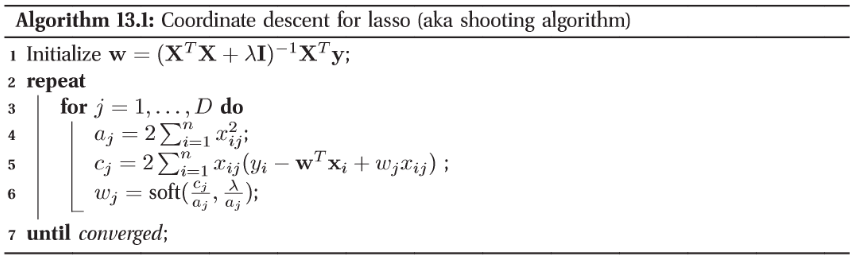
\includegraphics[width=1\textwidth]{shooting_algo} (Source: Murphy,
Kevin P. Machine learning: a probabilistic perspective. MIT press,
2012.) 
\par\end{center}

The ``soft thresholding'' function is defined as
\[
\text{soft}\left(a,\delta\right)=\text{sign}(a)\left(\left|a\right|-\delta\right)_{+}.
\]
Note that Murphy is suggesting to initialize the optimization with
the ridge regession solution, though this is not necessary. 

The solution should have a sparsity pattern that is similar to the
ground truth. Estimators that preserve the sparsity pattern (with
enough training data) are said to be \textbf{``sparsistent}\footnote{Li, Yen-Huan, et al. ``Sparsistency of $\ l_{1}$-Regularized $M$-Estimators.''}\textbf{''}
(sparse + consistent). Formally, an estimator $\hat{\beta}$ of parameter
$\beta$ is said to be consistent if the estimator $\hat{\beta}$
converges to the true value $\beta$ in probability as our sample
size goes to infinity. Analogously, if we define the support of a
vector $\beta$ as the indices with non-zero components, i.e. $\text{Supp}(\beta)=\{j\mid\beta_{j}\neq0\}$,
then an estimator $\hat{\beta}$ is said to be sparsistent if as the
number of samples becomes large, the support of $\hat{\beta}$ converges
to the support of $\beta$, or ${\displaystyle \lim_{m\rightarrow\infty}P[\text{Supp}(\hat{\beta}_{m})=\text{Supp}(\beta)]}$
= 1. 

There are a few tricks that can make selecting the hyperparameter
$\lambda$ easier and faster. First, you can show that for any $\lambda>2\|X^{T}(y-\bar{y})\|_{\infty}$,
the estimated weight vector $\hat{w}$ is entirely zero, where $\bar{y}$
is the mean of values in the vector $y$, and $\|\cdot\|_{\infty}$
is the infinity norm (or supremum norm), which is the maximum absolute
value of any component of the vector. Thus we need to search for an
optimal $\lambda$ in $\left[0,\lambda_{\text{max}}\right]$, where
$\lambda_{\text{max}}=2\|X^{T}(y-\bar{y})\|_{\infty}$. (Note: This
expression for $\lambda_{\text{max}}$ assumes we have an unregularized
bias term in our model. That is, our decision functions are $h_{w,b}(x)=w^{T}x+b$.
For the experiments, you can exclude the bias term, in which case
$\lambda_{\text{max}}=2\|X^{T}y\|_{\infty}$.)

Second, we can make use of the fact that when $\lambda$ and $\lambda'$
are close, so are the corresponding solutions $\hat{w}(\lambda)$
and $\hat{w}(\lambda')$. Start by finding $\hat{w}(\lambda_{\text{max}})$
and initialize the optimization at $w=0$. Next, $\lambda$ is reduced
(e.g. by a constant factor), and the optimization problem is solved
using the previous optimal point as the starting point. This is called
\textbf{warm starting} the optimization. The entire technique of computing
a set of solutions for a chain of nearby $\lambda$'s is called a
\textbf{continuation }or\textbf{ homotopy method}. In the context
of finding a good regularization hyperparameter, it may be referred
to as a \textbf{regularization path }approach. (Lots of names for
this!) 


\subsection{Experiments with the Shooting Algorithm}
\begin{enumerate}
\item Write a function that computes the Lasso solution for a given $\lambda$
using the shooting algorithm described above. This function should
take a starting point for the optimization as a parameter. Run it
on the dataset constructed in (1.1), and select the $\lambda$ that
minimizes the square error on the validation set. Report the optimal
value of $\lambda$ found, and the corresponding test error. Plot
the validation error vs $\lambda$. {[}Don't use the homotopy method
in this part, as we want to measure the speed improvement of homotopy
methods in part \ref{enu:homotopy}. Also, no need to vectorize the
calculations until part \ref{enu:vectorization}, where again we'll
compare the speedup. In any case, having two different implementations
of the same thing is a good way to check your work.{]}
\item Analyze the sparsity of your solution, reporting how many components
with true value zero have been estimated to be non-zero, and vice-versa. 
\item \label{enu:homotopy}Implement the homotopy method described above.
Compare the runtime for computing the full regularization path (for
the same set of $\lambda$'s you tried in the first question above)
using the homotopy method compared to the basic shooting algorithm.
\item \label{enu:vectorization}The algorithm as described above is not
ready for a large dataset (at least if it has been implemented in
basic Python) because of the implied loop over the dataset (i.e. where
we sum over the training set). By using matrix and vector operations,
we can eliminate the loops. This is called ``vectorization'' and
can lead to dramatic speedup in languages such as Python, Matlab,
and R. Derive matrix expressions for computing $a_{j}$ and $c_{j}$.
(Hint: A matlab version of this vectorized method can be found here:
\url{http://pmtk3.googlecode.com/svn-history/r1393/trunk/toolbox/Variable_selection/lassoExtra/LassoShooting.m}).
Implement the matrix expressions and measure the speedup to compute
the regularization path. 
\end{enumerate}

\subsection{Deriving the Coordinate Minimizer for Lasso}

This problem is to derive the expressions for the coordinate minimizers
used in the Shooting algorithm. This is often presented using subgradients
(e.g. \url{http://davidrosenberg.github.io/ml2015/docs/2.Lab.subgradient-descent.pdf#page=15}),
but here we will walk you through a bare hands approach (which is
essentially equivalent). 

In each step of the shooting algorithm, we would like to find the
$w_{j}$ minimizing
\begin{eqnarray*}
f(w_{j}) & = & \sum_{i=1}^{n}\left(w^{T}x_{i}-y_{i}\right)^{2}+\lambda\left|w\right|_{1}\\
 & = & \sum_{i=1}^{n}\left[w_{j}x_{ij}+\sum_{k\neq j}w_{k}x_{ik}-y_{i}\right]^{2}+\lambda\left|w_{j}\right|+\lambda\sum_{k\neq j}\left|w_{k}\right|,
\end{eqnarray*}
where we've written $x_{ij}$ for the $j$th entry of the vector $x_{i}$.
This function is strictly convex in $w_{j}$, and thus it has a unique
minimum. Furthermore, the only thing keeping $f$ from being differentiable
is the term with $\left|w_{j}\right|$. So $f$ is differentiable
everywhere except $w_{j}=0$. We'll break this problem into 3 cases:
$w_{j}>0$, $w_{j}<0$, and $w_{j}=0$. In the first two cases, we
can simply differentiate $f$ w.r.t. $w_{j}$ to get optimality conditions.
For the last case, we'll use the following more bare-hands characterization:
Since $f$ is convex, 0 is a minimizer of $f$ iff
\[
\lim_{\eps\downarrow0}\frac{f(\eps)-f(0)}{\eps}\ge0\quad\mbox{and}\quad\lim_{\eps\downarrow0}\frac{f(-\eps)-f(0)}{\eps}\ge0.
\]
This is a special case of the optimality conditions described in this
slide \url{http://davidrosenberg.github.io/ml2015/docs/5.Lab.misc.pdf#page=10},
where now the ``direction'' $v$ is simply taken to be the scalars
$1$ and $-1$, respectively. 
\begin{enumerate}
\item Give an expression for the derivative $f(w_{j})$ for $w_{j}\neq0$.
It will be convenient to write your expression in terms of the following
definitions:
\begin{eqnarray*}
\sign(w_{j}) & := & \begin{cases}
1 & w_{j}>0\\
0 & w_{j}=0\\
-1 & w_{j}<0
\end{cases}\\
a_{j} & := & 2\sum_{i=1}^{n}x_{ij}^{2}\\
c_{j} & := & 2\sum_{i=1}^{n}x_{ij}\left(y_{i}-\sum_{k\neq j}w_{k}x_{ik}\right).
\end{eqnarray*}

\item If $w_{j}>0$ and minimizes $f$, then show that $w_{j}=-\frac{1}{a_{j}}\left(\lambda-c_{j}\right)$.
Similarly, if $w_{j}<0$ and minimizes $f$, show that $w_{j}=\frac{1}{a_{j}}\left(\lambda+c_{j}\right)$.
Give conditions on $c_{j}$ that imply the minimizer $w_{j}>0$ and
$w_{j}<0$, respectively.
\item Derive expressions for the two one-sided derivatives at $f(0)$, and
show that $c_{j}\in\left[-\lambda,\lambda\right]$ implies that $w_{j}=0$
is a minimizer.
\item Conclude that the minimizer is given by
\[
w_{j}=\begin{cases}
\frac{1}{a_{j}}\left(c_{j}-\lambda\right) & c_{j}>\lambda\\
0 & c_{j}\in[-\lambda,\lambda]\\
\frac{1}{a_{j}}\left(c_{j}+\lambda\right) & c_{j}<-\lambda
\end{cases}
\]
 and show that this is equivalent to the expression given in \ref{sub:Shooting-algorithm}.
\end{enumerate}

\section{Lasso Properties}


\subsection{Deriving $\lambda_{\mbox{max}}$}

Show that for any $\lambda>2\|X^{T}(y-\bar{y})\|_{\infty}$, the estimated
weight vector $\hat{w}$ is entirely zero, where $\bar{y}$ is the
mean of values in the vector $y$, and $\|\cdot\|_{\infty}$ is the
infinity norm (or supremum norm), which is the maximum absolute value
of any component of the vector. {[}Hint: One approach is the following:
Suppose that $\hat{w}=0$ is a minimizer of the Lasso objective function.
Since the Lasso objective is convex, the one-sided directional derivative
must be nonnegative in every direction at $\hat{w}=0$. (See slide
\url{http://davidrosenberg.github.io/ml2015/docs/5.Lab.misc.pdf#page=10}.){]}


\subsection{{[}Optional{]} Feature Correlation}

In this problem, we will examine and compare the behavior of the Lasso
and ridge regression in the case of an exactly repeated feature. That
is, consider the design matrix $X\in\reals^{m\times d}$, where $X_{\cdot i}=X_{\cdot j}$
for some $i$ and $j$, where $X_{\cdot i}$ is the $i^{th}$ column
of $X$. We will see that ridge regression divides the weight equally
among identical features, while Lasso divides the weight arbitrarily.
In an optional part to this problem, we will consider what changes
when $X_{\cdot i}$ and $X_{\cdot j}$ are highly correlated (e.g.
exactly the same except for some small random noise) rather than exactly
the same. 
\begin{enumerate}
\item {[}Optional{]} Derive the relation between $\hat{\theta}_{i}$ and
$\hat{\theta}_{j}$, the $i^{th}$ and the $j^{th}$ components of
the optimal weight vector obtained by solving the Lasso optimization
problem. \\
{[}Hint: Assume that in the optimal solution, $\hat{\theta}_{i}$
= $a$ and $\hat{\theta}_{j}$ = $b$. First show that $a$ and $b$
must have the same sign. Then, using this result, rewrite the optimization
problem to derive a relation between $a$ and $b$.{]} 
\item {[}Optional{]} Derive the relation between $\hat{\theta}_{i}$ and
$\hat{\theta}_{j}$, the $i^{th}$ and the $j^{th}$ components of
the optimal weight vector obtained by solving the ridge regression
optimization problem. 
\item {[}Optional{]} What do you think would happen with Lasso and ridge
when $X_{\cdot i}$ and $X_{\cdot j}$ are highly correlated, but
not exactly the same. You may investigate this experimentally or geometrically.
\end{enumerate}

\section{The Ellipsoids in the $\ell_{1}/\ell_{2}$ regularization picture}

Recall the famous picture purporting to explain why $\ell_{1}$ regularization
leads to sparsity, while $\ell_{2}$ regularization does not. Here's
the instance from Hastie et al's \emph{The Elements of Statistical
Learning:}

\begin{center}
\includegraphics[width=0.5\paperwidth]{L1-L2-corner-pic-ESL-Fig3\lyxdot 11} 
\par\end{center}

(While Hastie et al. use $\beta$ for the parameters, we'll continue
to use $w$.) 

In this problem we'll show that the level sets of the empirical risk
are indeed ellipsoids centered at the empirical risk minimizer $\hat{w}$.

Consider linear prediction functions of the form $x\mapsto w^{T}x$.
Then the empirical risk for any $w$, the empirical risk for $f(x)=w^{T}x$
under the square loss is
\begin{eqnarray*}
\hat{R}_{n}(w) & = & \frac{1}{n}\sum_{i=1}^{n}\left(w^{T}x_{i}-y_{i}\right)^{2}\\
 & = & \frac{1}{n}\left(Xw-y\right)^{T}\left(Xw-y\right).
\end{eqnarray*}

\begin{enumerate}
\item Let $\hat{w}=\left(X^{T}X\right)^{-1}X^{T}y$. Show that $\hat{w}$
has empirical risk given by 
\[
\hat{R}_{n}(\hat{w})=\frac{1}{n}\left(-y^{T}X\hat{w}+y^{T}y\right)
\]

\item \label{enu:emprisk-ellipsoid}Show that for any $w$ we have
\[
\hat{R}_{n}(w)=\frac{1}{n}\left(w-\hat{w}\right)^{T}X^{T}X\left(w-\hat{w}\right)+\hat{R}_{n}(\hat{w}).
\]
Note that the RHS (i.e. ``right hand side'') has one term that's
quadratic in $w$ and one term that's independent of $w$. In particular,
the RHS does not have any term that's linear in $w$. On the LHS (i.e.
``left hand side''), we have $\hat{R}_{n}(w)=\frac{1}{n}\left(Xw-y\right)^{T}\left(Xw-y\right)$.
After expanding the out, you'll have terms that are quadratic, linear,
and constant in $w$. Completing the square is the tool for rearranging
an expression to get rid of the linear terms. The following ``completing
the square'' identity is easy to verify just by multiplying out the
expressions on the RHS:
\begin{eqnarray*}
x^{T}Mx-2b^{T}x & = & \left(x-M^{-1}b\right)^{T}M(x-M^{-1}b)-b^{T}M^{-1}b
\end{eqnarray*}
 
\item Using the expression derived for $\hat{R}_{n}(w)$ in \ref{enu:emprisk-ellipsoid},
give a very short proof that $\hat{w}=\left(X^{T}X\right)^{-1}X^{T}y$
is the empirical risk minimizer. That is: 
\[
\hat{w}=\argmin_{w}\hat{R}_{n}(w).
\]
Hint: Note that $X^{T}X$ is positive semidefinite and, by definition,
a symmetric matrix $M$ is positive semidefinite iff for all $x\in\reals^{d}$,
$x^{T}Mx\ge0$.
\item Give an expression for the set of $w$ for which the empirical risk
exceeds the minimum empirical risk $\hat{R}_{n}(\hat{w})$ by an amount
$c>0$. This set is an ellipse -- what is its center?
\end{enumerate}

\section{{[}Optional{]} Projected SGD via Variable Splitting}

In this question, we consider another general technique that can be
used on the Lasso problem. We first use the variable splitting method
to transform the Lasso problem to a smooth problem with linear inequality
constraints, and then we can apply a variant of SGD.

Representing the unknown vector $\theta$ as a difference of two non-negative
vectors $\theta^{+}$ and $\theta^{-}$, the $\ell{}_{1}$-norm of
$\theta$ is given by ${\displaystyle \sum_{i=1}^{d}{\theta_{i}^{+}}}$
+ ${\displaystyle \sum_{i=1}^{d}{\theta_{i}^{-}}}$. Thus, the optimization
problem can be written as 
\begin{gather*}
(\hat{\theta}^{+},\hat{\theta}^{-})={\displaystyle \argmin_{\theta^{+},\theta^{-}\in\reals^{d}}{\sum_{i=1}^{m}{(h_{\theta^{+},\theta^{-}}(x_{i})-y_{i})^{2}}}+\lambda\sum_{i=1}^{d}{\theta_{i}^{+}}+\lambda\sum_{i=1}^{d}{\theta_{i}^{-}}}\\
\mbox{such that }\theta^{+}\ge0\mbox{ and }\theta^{-}\ge0,
\end{gather*}
where $h_{\theta^{+},\theta^{-}}(x)=(\theta^{+}-\theta^{-})^{T}x$.
The original parameter $\theta$ can then be estimated as $\hat{\theta}=(\hat{\theta}^{+}-\hat{\theta}^{-})$.

This is a convex optimization problem with a differentiable objective
and linear inequality constraints. We can approach this problem using
projected stochastic gradient descent, as discussed in lecture. Here,
after taking our stochastic gradient step, we project the result back
into the feasible set by setting any negative components of $\theta^{+}$
and $\theta^{-}$ to zero.
\begin{enumerate}
\item {[}Optional{]} Implement projected SGD to solve the above optimization
problem for the same $\lambda$'s as used with the shooting algorithm.
Since the two optimization algorithms should find essentially the
same solutions, you can check the algorithms against each other. Report
the differences in validation loss for each $\lambda$ between the
two optimization methods. (You can make a table or plot the differences.) 
\item {[}Optional{]} Choose the $\lambda$ that gives the best performance
on the validation set. Describe the solution $\hat{w}$ in term of
its sparsity. How does the sparsity compare to the solution from the
shooting algorithm? \end{enumerate}

\end{document}
